\chapter{Introduction}
\pagenumbering{arabic}
\setcounter{page}{1}
\section{Background}
The Norwegian economy is cooling under a pessimistic oil price of close to 37 USD per barrel as of December 2015. Under heavy pressure to perform, companies involved in the exploitation of hydrocarbons are cutting costs while trying to increase productivity.

As a means of improving profitability, real-time decision support systems have been developed. One example of these was a product of work done at NTNU, by Verdande Technology, established 2004. The company is now closed down after becoming bankrupt in December 2014 as potential customers were cutting costs.

Automation of pipe handling have been pursued by several companies in the oil rig equipment production market with moderate success. The industry have realized that more may be gained from supporting humans in the center of the operation, than to completely eliminate humans. As such, systems to support the human driller need to be developed.

Support systems that may improve safety and productivity includes improvements to the graphical user interface, presentation of relevant and aggrevated data, as well as integrated camera systems.

The main objective of this MSc thesis is to implement a system that provides a better situation overview through automated CCTV tracking of machines.

This MSc thesis should address the following:
\begin{itemize}
\item Implementation of an auto tracking CCTV system using glyphs as visual descriptor.
\item Analysis of dataset with real-world weather over a long period.
\item Prototyping of an implementation to detect casings and pipes in a fingerboard.
\end{itemize}

\subsection{Problem formulation}
How can computer vision assisted camera tracking be exploited to increase safety and situational awareness in any process involving heavy machinery and remote operation?

How will GPU-acceleration of the computer vision algorithm affect the system?

How can we reduce the latency of the live camera feed to make feedback control of the camera better?

How can we track an object across multiple cameras?

How can we identify tubulars in a fingerboard using machine vision, so that the control system can verify its data?

The end goal is to reduce the possibility of an undesired event, be it either damage to humans or expensive equipment, and increase speed of operations.

\subsection{Literature survey}
As discussed by \citet{sklet05}, the concept of a safety barrier is not clearly defined and its meaning is ambiguous. With this in mind, we are looking to implement what \citet{rausand14} describes as a proactive safety barrier, also known as a frequency-reducing barrier, in other words a system to reduce the frequency of undesired events.

Semi-automated CCTV surveillance have been considered by \citet{dadashi12} as a method of increasing the capacity of a human operator in a traditional human surveillance situation. The reliability for fully automated systems were not considered good enough for an operator to trust. The findings recommend providing feedback about system confidence and accuracy to the operator, which makes the automated component of such a system more 'visible' to its user. For the case of this thesis, the act of displaying visual cues overlaid on the CCTV images are considered. This would hopefully increase trust, and expose the automated component of our fully automated tracking system.

The machine vision algorithm that was implemented in the authors earlier work, as mentioned in work done by \citet{boyers13} and \citet{kirillov10}, will be used to recognize the distinct symbol, hereafter called a glyph.

The challenges of outdoor machine vision in uncontrollable weather and lightning conditions have been raised by the author in the same unpublished project thesis. Figure \ref{fig:timelapse_viewpoint} shows a series of images captured by the author, which shows the differences in color, clarity and reflections.

\begin{figure}[ht]
    \centering
    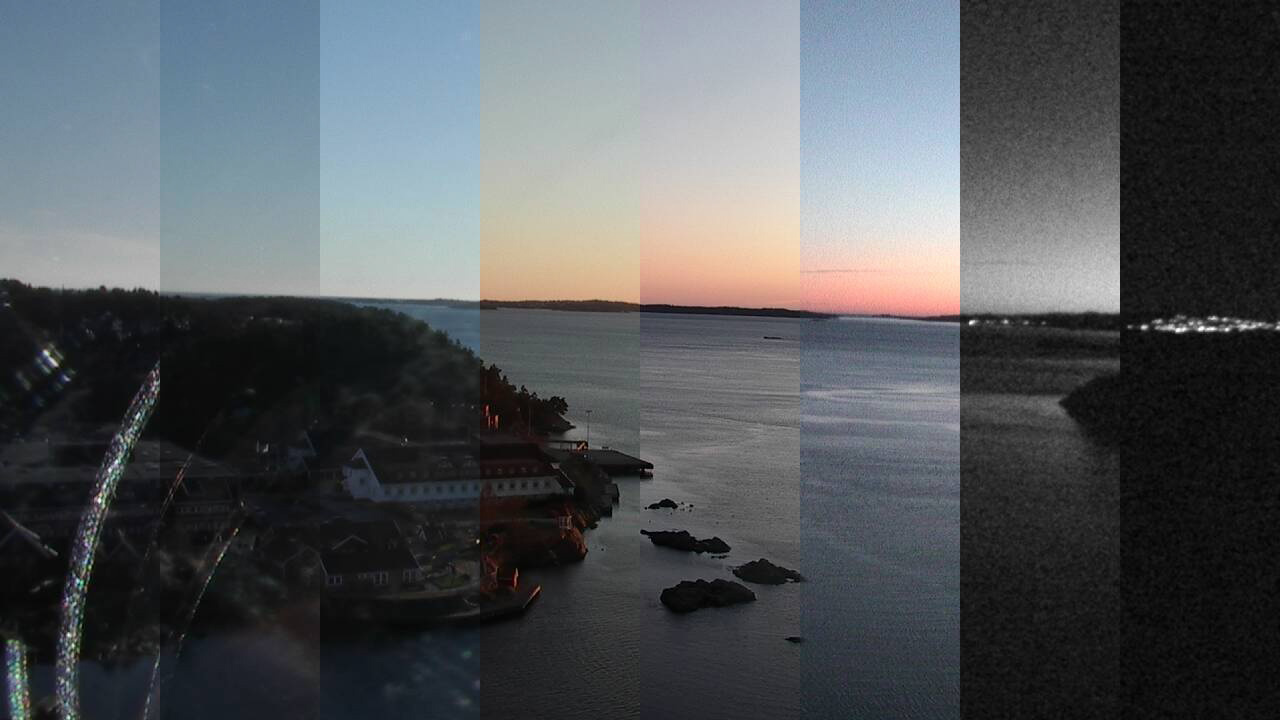
\includegraphics[width=1.0\textwidth]{timelapse_viewpoint.jpg}
    \caption{Timelapse through a day of a CCTV camera in Kristiansand, 4th of March 2015. Source: Own work}
    \label{fig:timelapse_viewpoint}
\end{figure}
\FloatBarrier

Our camera of choice, an AXIS Q6045 was selected both by its widespread use in the oil- and gas industry, and because this is what the author had at hand. It is a modern high-definition PTZ-camera produced by Axis Communications.  Axis Communications have provided a white paper which provides a good overview of the various elements that increase latency in a live video stream. This document is available online. \citep{axis15}

The inherit differences between analog and digital IP\footnote{IP, the short form of Internet Protocol, a principal communications protocol for relaying datagrams across network boundaries. IPv4 was deployed in the ARPANET in 1983.} transmission of video have been examined by \citet{hill09}, and the conclusion was that latency present in digital IP transmission is within acceptable values for normal usage. Still, the article presents findings that show latency of a digital transmission being more than 5x of the analog transmission latency. The latency was measured to be between 120 ms up to 1600 ms depending on the resolution of the image and its compression. The upsides of digital transmission include increased quality of image, flexibility of digital encoding and ability to use analytic software. The paper does not describe other forms of digital video transmissions that exist, including raw digital transmission using SDI\footnote{Serial Digital Interface, high-speed digital video transmission defined by Society of Motion Picture \& Television Engineers.}, and it is also outdated in terms of the current state of the art cameras available, but it provides a reference.

Work done by \citet{svensson13} involved methods to reduce the delays that are inherently found in digital IP transmission systems and the control of these. Their research was done on AXIS Q6035 and AXIS Q6032 cameras. The author assumes these to be closely related to the AXIS Q6045, and their findings therefore useful for work done in this thesis. Findings include camera operating system being among the key factors for video delay, as the stock cameras have implemented an inefficient communication scheme, and there are other suggestions to reduce delay presented. For the scope of this thesis, we will have these delays in mind and build around them, as any operating system upgrades have to come from Axis themselves if any company would consider using them.

Tracking of objects across multiple cameras have been explored with most focus on overlapping camera views. Some work has also been done on non-overlapping camera views by \citet{javed03}, where camera topology and path probabilities are learnt without any inter-camera calibration. When images from several sources are used, the time-synchronization of the images becomes crucial as a point of reference. Through the use of Parzen windows, the inter-camera space-time probabilities can be mapped. The method mentioned does require a learning phase.

\subsection{What remains to be done?}
As a summary of the literature survey, we see that much work has been done in the different fields, but not much have been found on combining the results of these into a solution that can provide modern, automated CCTV tracking of industrial processes involving heavy machinery in a way that retains the human operator in the center of the process.

The implementation and comparison of a robust and responsive automated CCTV tracking system remains to be done, as an earlier proof of concept implementation was done by the author in 2014.

Not much literature on fingerboard tubular detection have been found. It is believed that the reason for this is that the word fingerboard is a technical jargon used in the drilling industry, and that any research done is done in-house with no intention of publishing results.

The implementation of a simple fingerboard tubular detection program remains to be done, and the analysis of its performance.

We aim to combine as much as possible from the various fields, given constraints of time, into a proof of concept which can be the stepping stone to a commercial product in the case of CCTV tracking, and a prototype implementation for the fingerboard tubular detection.

\section{Objectives}
The objectives of the work done through this thesis consists of:
\begin{enumerate}
  \item Implementation of a multi-source GPU-accelerated machine vision program that can control a CCTV camera and follow a glyph symbol, and comparison of its performance
  \item Implementation of a proof of concept tubular-detection program for fingerboards
\end{enumerate}

\section{Limitations}
The limitations that relates to this study includes both technical challenges, environmental and operational conditions, but focus is on the technical challenges for the sake of brevity.

As CCTV cameras have evolved, the video transfer method has gone through some changes to cater for higher resolutions and more true representation of the world as observed. By this, analog signals have been replaced by digital signals. Analog transmission is known for being both robust, simple and near-instant, however they are prone to signal deterioration which may affect machine vision algorithms, and their flexibility of location is not as good as modern digital transmission. With digital transmission, commonly using IP, the cost of these systems have gone down, flexibility have gone up and resolution as well as control has improved, yet this have introduced new challenges. Packet loss is a real possibility in IP networks, increased latency through encoding and decoding of the video stream and a shared network highway puts more demand on the implementation. One serious limitation to the implementation of the system as presented, is therefore as a feedback system, the upper latency limit for which when the system becomes unstable. The use of raw digital transmission such as SDI would minimize latency and give room for even higher resolution images with little to no chance of data loss, but this has not been explored as it requires specialized cameras, coaxial cables and frame grabbers.

Technology is highly guarded, and real offshore operations are not easy to get access to. Cooperation is not common in the industry, and transparency of systems and solutions may be less than ideal. This limits the available data set for the purpose of research and making robust systems.

The software world progress quickly, and new solutions can suddenly become obsolete. The technological debt increases quickly. This would make an externally maintained solution seem like a better idea, but sharing information to make the development work is not an easy task as each company protects its own interests.

Heterogeneous computing platforms are still considered to be in its infancy, and both CUDA as well as OpenCL is under active developement. Choosing one technology will lead to an exclusion of either benefits or available computing platforms. A limitation here is that the resulting speed and benefits of heterogeneous computing are not set in stone, and that there will always be improvements that can be done to make an otherwise unworkable system become a successful implementation.

Algorithms implemented will not be robust enough to handle all possible lightning conditions, and some of these may assume that a certain color can be identified. This means that artificial lightning is paramount for reliable machine vision outdoors, if we are to only rely on optical sensors. Alternatives exist, but these will not be explored further in this thesis. The author have made a summary of these that can be read in the unpublished project thesis \citet{joakimsk14}.

It is considered a hard challenge to make a truly reliable system that works in the real world. Making a tabletop solution is not nearly enough to allow a big company to test this offshore at a customers platform, and much work remains before a fully commercial solution is ready for sale.

Seeing past these limitations, however, is a world of possibilities, which this study intends to explore.

\section{Approach}
\subsection{CCTV tracking system}
The implementation of the CCTV tracking system will be based on the authors previous work and be written in C++ with heterogeneous support from a GPU to increase performance.

After this system has been built, it will be tested with and without GPU acceleration, to determine if the full solution becomes more stable and reliable.

A data-set will be analyzed to test the robustness of the machine vision implementation and comment how snow, sun and other real-world factors affect the output.

It will also be tried to use multiple video sources, however due to the lack of several CCTV cameras, this will only partially be explored using a common webcamera, as a means of doing camera handover.

\subsection{Pipe detection system}
The construction of a proof of concept pipe detection system for fingerboards will be done in a rapid prototyping environment, to show that it is possible to increase control system awareness in existing infrastructure on the oil rig.

\section{Structure of the report}
All the software developed as a part of this project can be found at the authors personal repository at Github, ~\cite{github}, feel free to use this for future non-commercial work. The Latex source is also available. Some information may have been omitted to hide confidential company information.

\section{Structure of the DVD}
The DVD contains a snapshot of the latest Github code repository as of the date of this report.